\section{Hysteresis}
\label{sec:hysteresis}

The final step in the Canny edge detection algorithm is edge linking through a process called \emph{hysteresis}. This step aims to connect weak edge pixels to strong edge pixels to form continuous and complete edges in the image.

What hysteresis does is, it helps to eliminate false edges by considering the connectivity of weak edges to strong edges. The idea is that if a weak edge pixel is connected to a strong edge pixel, it should be retained as part of the edge. Conversely, if a weak edge pixel is not connected to any strong edge pixels, it should be discarded.

The hysteresis process involves the following steps:

\begin{enumerate}
    \item Examine a weak edge pixel and its 8-connected neighborhood pixels.
    \item Identify if there is at least one strong edge pixel in the neighborhood.
    \item If a strong edge pixel is found, preserve the weak edge pixel as part of the edge, i.e., convert it to a strong edge pixel.
    \item Repeat the process for neighboring weak edge pixels to ensure continuity.
\end{enumerate}

The visualization of the hysteresis process is shown in \autoref{fig:hysteresis-example}. In the first case, the weak edge pixel has no strong edge neighbors, so it is set to 0. In the second case, the weak edge pixel has (at least one) strong edge neighbors, so it is set to 255.

\begin{figure}[ht]
    \centering
    \begin{subfigure}[b]{0.4\textwidth}
        \centering
        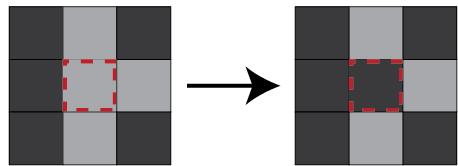
\includegraphics[width=0.9\textwidth]{hysteresis-no-strong-around.png}
        \caption{Weak Pixel with No Strong Neighbors (Set to 0)}
        \label{fig:hysteresis-no-strong-around}
    \end{subfigure}
    \hfill
    \begin{subfigure}[b]{0.4\textwidth}
        \centering
        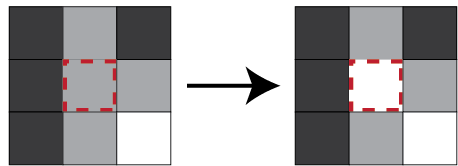
\includegraphics[width=0.9\textwidth]{hysteresis-one-strong-around.png}
        \caption{Weak Pixel with Strong Neighbors (Set to 255)}
        \label{fig:hysteresis-one-strong-around}
    \end{subfigure}
    \caption{Effect of Hysteresis on Weak Edge Pixels}
    \label{fig:hysteresis-example}
\end{figure}

The result of the hysteresis process is a binary image with strong edges that are connected to weak edges, forming complete edges in the image, as shown in \autoref{fig:hysteresis}.

\begin{figure}[ht]
    \centering
    \begin{subfigure}[b]{0.4\textwidth}
        \centering
        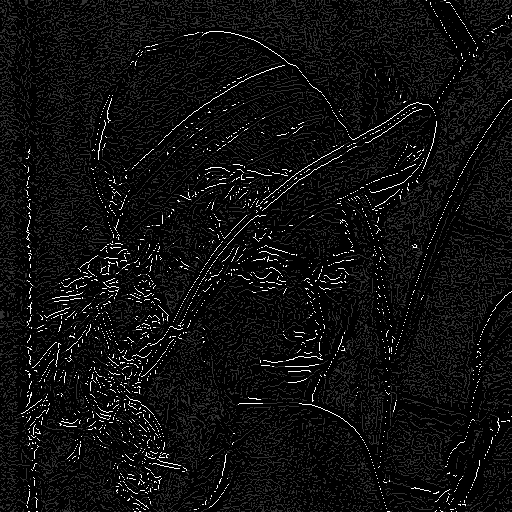
\includegraphics[width=0.9\textwidth]{lenna_7_double_thresholded.png}
        \caption{After Double Thresholding}
    \end{subfigure}
    \hfill
    \begin{subfigure}[b]{0.4\textwidth}
        \centering
        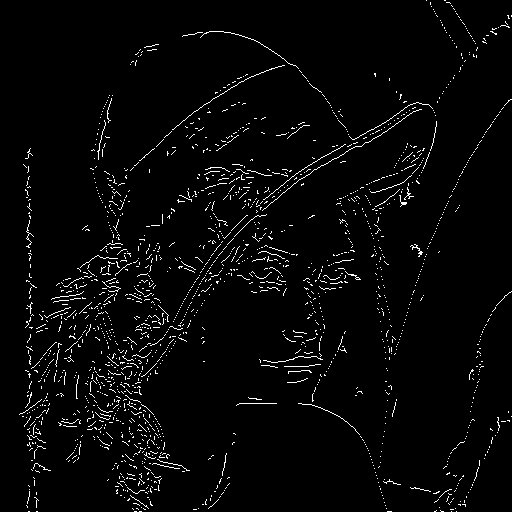
\includegraphics[width=0.9\textwidth]{lenna_8_canny_edge_detected.png}
        \caption{After Hysteresis}
    \end{subfigure}
    \caption{Effect of Hysteresis}
    \label{fig:hysteresis}
\end{figure}
